\section{Introduction}

When connecting two rotary mechanical devices a coupler is used to connect them. These include the use of 1:1 flexible shaft couplers, to compensate for possible shaft misalignments, as well as belts, and gear boxes. In theory it is desired to have the given coupler be perfectly rigid, ever degree the actuator turns the connected load will turn to its exact location denoted by the input and the gear ratio. For a coupler to be perfectly rigid the latter must be true for all time. In reality gear boxes and couplers are not perfectly rigid and have spring and damping terms associated with them. The spring constant causes the system to have two resonant frequencies collectively called the Torsional Resonance (TR). The TR frequencies, which are referred to as the resonant frequency, wr, and the anti-resonant frequency, war, can not fall within the pass- band of the closed loop servo because it will cause instability.Figure 1 shows a diagram of an ideal coupled system (Left) and a system exhibiting TR (Right). The ideal system can be reduced to a single acting inertia of Ja+JL while the system exhibiting TR is connected by a spring damper system thus that reduction can not be made.

\begin{figure}[t]
  \centering
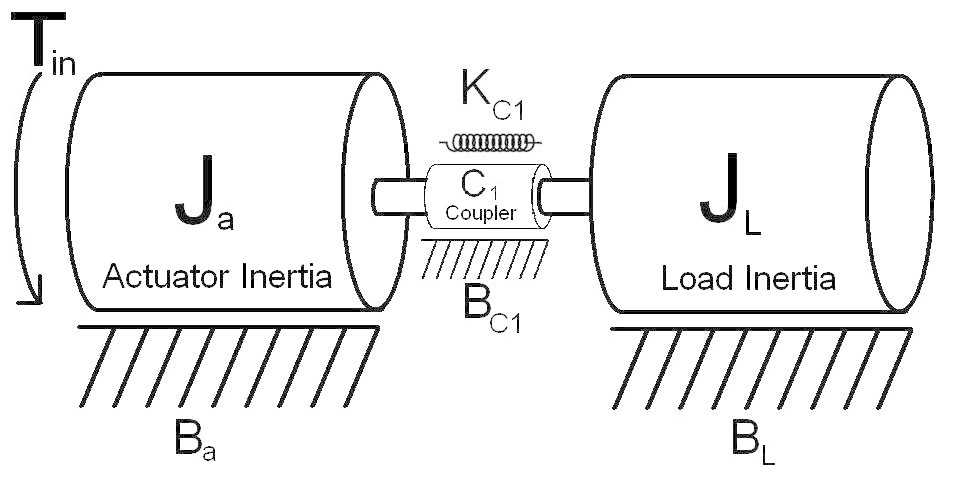
\includegraphics[width=1.0\columnwidth]{./pix/couple.png}
  \caption{System exhibiting TR. In an ideal
system (without TR) the load can be represented as a single acting inertia $(J_a+J_L)$.  The system exhibiting TR is connected by a
spring damper system thus that reduction can not be mad}
  \label{fig:couple}
\end{figure}


The ideal frequency response of the ideal coupled system, with ?a as the output and Tin as the input, can be found in Figure 2 on the left graph. The magnitude portion of the frequency response is a straight line with a slope of negative 40dB/dec. The phase of the latter system does not change. The frequency response of the system exhibiting TR can be found in Figure 2 on the right plot. It can be noted that at resonance there is a peak. This peak reduces the gain margin of the system. The phase also changes around the resonance which reduces the phase margin.

Contemporary ways of reducing this problem include:
\begin{itemize}
\item  Reducing the servo�s bandwidth so it does not include the TR frequencies. (Appendix E)\item Increasing the couplers spring constant Kc via using higher quality and anti backlash mechanical couplers and gearboxes to push the TR frequencies higher. (Appendix G)
\item Using notch filters to reduce the resonant peak. (Appendix D)
\end{itemize}

Reducing the bandwidth of the servo means that the designed system will not be able to respond as quickly to an input stimulus. Using higher quality and anti-backlash mechanical couplers and gearboxes will give you greater bandwidth but will also include a higher materials price tag. It is also important to note that the use of notch filters is only useful in systems where the TR does not change. Most systems that have TR present tend to have nonlinear, and time varying, elements, including dynamic loads, that will cause the TR frequency to change thus making the notch filter less effective in the ideal case.

\subsection{Designs to be Considered: Resonance Equalization}
W. J. Bigley and V. Rizzo presented a technique for, as they describe it, �eliminating the destabilizing effect of mechanical resonance in feedback control systems.� [1] The goal of their research was to make a wide band high performance closed loop servo system. In their research Bigley and Rizzo found a relationship between the torque, or current, on the DC motor and the velocity of the shaft. They found that when the current is at its maximum the velocity is at a minimum, no matter where the resonance or anti resonance occurs, see Figure 27. Thus feeding back the velocity and torque states would compensate for the effects of TR no matter where it occurs even when the parameters of the system changes.

\subsection{Designs to be Considered: Sliding Mode Control}
Sliding mode control (SMC) is also a good candidate for a method to reduce the effects of TR. This isbecause SMC is a robust control method that is able to properly control a system even when parameters are not precisely known. The main idea about SMC is that you are able to make a control that will guarantee the performance of a system in u and x, see Figure 31, within a given error ? and ? respectively. When using SMC one, or more, parameters are chosen to be unknown. The unknown parameters are given a range that they are able to be between and still have the system perform properly.






